\hsection{Compact Crow's Foot Notation}%
\label{sec:compactCrowsFootNotation}%
%
From \cref{fig:erdPersonStudentFaculty2}, we can draw two very general conclusions about the notation we used (entities as rectangles, attributes as ellipses, and relationships as diamonds, combined with the Crow's Foot method for expression cardinalities):
First, it indeed allows us to model real-world situations as datastructures and their relationships.
Second, it is also a bit verbose.
Especially if we have many attributes, the ellipses get many and hard to read.
The diamonds to expression relationships are also space consuming.

There also is a more compact method to express (almost) the same information:
We can combine \pgls{UML} class diagrams with the Crow's Foot notation as well.
This is a very commonly used method in several tools.
Let us investigate it here and use it to further explore our example application, the teaching management platform.
%
\begin{figure}%
\centering%
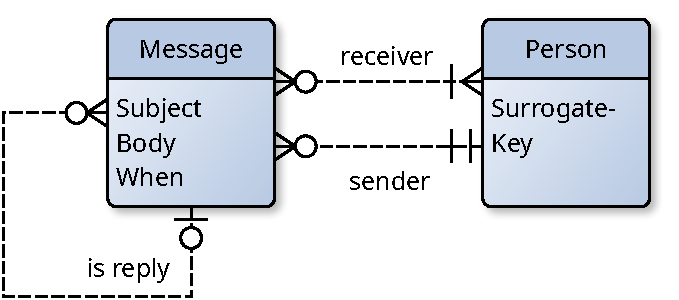
\includegraphics[scale=0.6]{\currentDir/erdMessage1}%
\caption{The structure of the messaging subsystem of the teaching management platform.}%
\label{fig:erdMessage1}%
\end{figure}%
%
In \cref{fig:erdMessage1}, we sketch the messaging subsystem of our teaching management platform.
In this notation, an entity type is still visualized a rectangle.
In the top part of the rectangle, the entity type name is written.
In the second part, we write the list of attributes.
As you remember, \emph{Person} is a strong entity type in our model.
The new entity type \emph{Message} is a strong entity type as well.
It as three attributes, \emph{Subject}, i.e., the title of the message, and \emph{Body}, i.e., the message text, and \emph{When}, the date and time when the message was sent.

Relationships in this visualization approach are modeled just as lines connecting the entities.
No diamonds are used, but instead the relationship names are written as labels directly adjacent to the lines.
Each message has exactly one person as sender.
Each person can be the sender of arbitrarily many messages.
Each message has at least one, but potentially many persons as receiver.
Each person can receive zero or arbitrarily many messages.
Additionally, a message can be the answer to no or exactly one (previous) message.
There can be arbitrarily many answers to each message.

Before, we signified strong and weak entities by using normal or double-lined rectangles.
Now, instead, relationships can be weak or strong~\cite{P2024C6DS:EM}.%
%
\begin{definition}[Identifying Relationship]%
A \emph{identifying} (strong) relationship is connected to at least one weak entity and is required for identifying the weak entity. %
\end{definition}%
%
Usually, a strong relationship connects a strong entity to a weak entity.
The weak entity cannot exist without the strong entity.
The primary key of the strong entity is then part of the key of weak entity.
Strong relationships are signified by solid lines.%
%
\begin{definition}[Non-Identifying Relationship]%
A \emph{non-identifying} (weak) relationship is not needed to identify an entity.%
\end{definition}%
Examples for this are, e.g., two connected strong entities.
But also weak entities can be connected, as long as the connection is not required for identifying purposes.

\begin{figure}%
\centering%
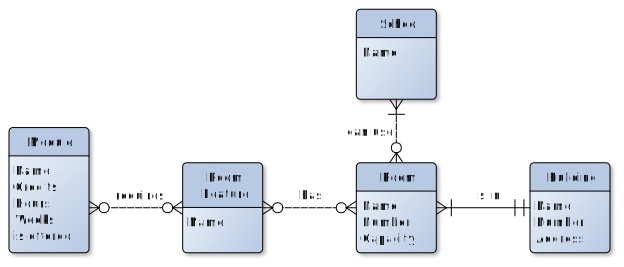
\includegraphics[scale=0.6]{\currentDir/erdRoom1}%
\caption{The room planning subsystem of the teaching management platform.}%
\label{fig:erdRoom1}%
\end{figure}%
%
We now develop the room management subsystem for our teaching management platform in \cref{fig:erdRoom1}.
In this model, buildings are strong entities.
They may have a name, maybe something like 合肥大学综合实验楼, and a number, let's say~53.
We also offer an address string.
No real addresses as discussed before are needed, because we certainly do not need to model countries or provinces here.
We assume that all classes of a curriculum take place in the same country, province, and city.
However, maybe the university has different campuses, like 南一区 and 南二区, which would be something useful to write there.

Rooms exist within buildings, so they are weak entities.
They have a number and maybe a name.
Each room has a capacity limit for students.
They are connected to the building entities via identifying relationships:
A room must be in exactly one building, whereas a building should consist of one or many rooms (otherwise, we do not need to store it in our \db).

The last sentence is interesting, as it poses a somewhat philosophical problem.
We said that \inQuotes{each room is inside one building and each building is composed of one or multiple rooms.}
This is what we wrote in our \pgls{ERD} in \cref{fig:erdRoom1} and this is what makes sense.
On a technical level, this causes me to scratch my head.
Regardless of what data model I use, I will be forced to instantiate the data structure for \emph{Room} to, well, represent a room in my \db.
Following the formal definition of the above rule, I would need to have an existing entity of type \emph{Building} at this point in time.
Because I must link each room to one building.
So I must first instantiate \emph{Building} and then I can instantiate \emph{Room}.
However, if I interpret my \pgls{ERD} strictly, I face the problem that each building must also be connected to at least one room.
So this means that I would first need an instance of \emph{Room} before I can instantiate the \emph{Building} entity type.

This philosophical dilemma, resulting from nitpicking, can be solved in three ways:
First, we could say:
\emph{\inQuotes{Well, the conceptual model represents the real world. %
In the real world, each room is inside a building and a building has at least one room. %
That is true and that is what we model here.
Whether or not this can be realized technically is not relevant at this stage of development.}}
Second, we could say, maybe even as a corollary of the above, that:
\emph{\inQuotes{On a technical level, we simply do not enforce that buildings must contain rooms. %
We know that the user will add rooms to buildings eventually. %
We just accept that there may be a temporary state of the \db\ where one of the mutual dependency constraints is violated. %
Just for a short time, between the moment when the user has created a building and right before she adds a room. %
It doesn't matter.}}

Third, we could even solve this technically:
Most \pglspl{dbms} support \emph{transactions}, i.e., groups of instructions to the \db\ that are executed as one atomic unit and either fail together or succeed together.
There is no intermediate state, as transactions are indivisible, atomically executed units.
Thus, we could require that every time a new building is added to the \db, the first room is specified as well.
The creation of the building and room record could be executed together as atomic transaction.
If we do this, the conceptual constraints would perfectly map to a technical constraints, at the expense of slightly more complex update operations~(because we now need to use transactions).
\postgresql\ permits us to defer the constraints checking to the end of a transaction via the \sqlil{SET CONSTRAINTS ALL DEFERRED}\sqlIdx{SET CONSTRAINTS} command~\cite{PGDG:PD:SC:SC,N2016SSFA:DC}.

Anyway.
Rooms are also connected with non-identifying relationships to schools:
One school may be permitted to use zero or more rooms for teaching.
Each room must be usable by at least one school (because otherwise, we simply don't need to store it in the \db).

We can easily expect that different teaching modules may have different requirements regarding the rooms.
For normal teaching, it may be sufficient that an overhead projector is present.
We could assume that this is always the case.
However, for practical computer science lab classes, we may need one computer per desk.
For chemistry experiment classes, we may need a smoke outlet and something for chemical waste disposal.
To model this, we create the strong entity \emph{Room Feature}, which just needs a descriptive name.
Rooms are linked via non-identifying connections to such features:
Each room may have zero or one or many such features.
Each room feature may be provided by zero, one, or many rooms.
At the same time, a teaching module may require any number of room features.
A room feature may be required by any number of teaching modules.

\begin{figure}%
\centering%
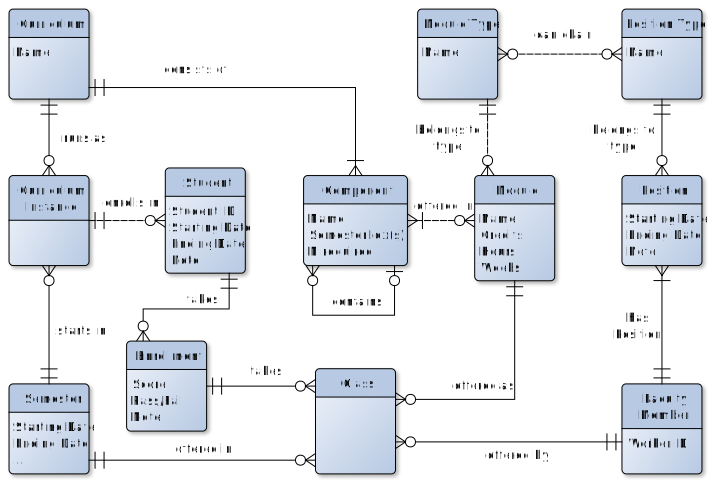
\includegraphics[width=0.99\linewidth]{\currentDir/erdModules1}%
\caption{A re-design of the student/curriculum/faculty/module interactions in our teaching management platform.}%
\label{fig:erdModules1}%
\end{figure}%
%
Let us now re-design the interactions of students, curricula, faculty, and modules.
Wen we initially discussed our plans for designing these systems, we discussed with our stakeholders in the university.
We learned that, for example, some abilities of teachers are bound to their position, e.g., which kind of modules they can chair.
Other abilities should be bound to their person, e.g., whether they can be Master's supervisor.
We did model this back in \cref{fig:erdPersonStudentFaculty2}.
There also are two different ways teachers and students can interact:
Students can enroll in classes of professors and/or a professor can be their BSc or MSc supervisor.
Basically, we would have two sets of interactions governed by two different forms credentials on the teacher's side.

We have the idea to unify them both in \cref{fig:erdModules1}.
It is clear that not all teachers can chair all types of modules.
Maybe our university will only permit full professors to chair core modules of a curriculum, while younger lecturers can propose and chair elective (voluntary) courses.
This can easily be covered by relating position types to module types.
Then again, some modules may require special certifications, such as chemistry safety certification or something.
This does not fit well to the position type-module type approach, because \inQuotes{chemistry safety certified} is not a position.
The same holds for \inQuotes{Master's Supervisor}.

Well, not necessarily:
How about we permit that a person can hold multiple positions at a time.
Besides the traditional positions, we could add things like \inQuotes{Chemistry Safety Certified,} \inQuotes{Master's Supervisor,} an whatever else we need.
That positions are limited by starting and ending dates is also not a problem.
This is exactly a feature that we would like to have.
Interestingly, with our \emph{Position} and \emph{Position Type} entity types used like this, we could easily represent even more complex functions, such as Dean, Vice-Dean for Teaching, Department Head, Team Head, and so on.
These functions could then be tied to what kind of changes the person can make to the data.

But back to the relationship between teaching and position.
Each \emph{Module Type} entity can now be linked to one or multiple \emph{Position Type}s that a teacher must hold to be permitted to chair them.
Each position type, of course, can be the credential for chairing modules of multiple different module types.
This approach works because we realize that Master's and Bachelor's projects are, basically, just special module types.
They would automatically be covered by this permission system.

A school in our university may offer different curricula, e.g., a Master of Computer Science or a Bachelor of Engineering in Computer Science.
Initially, we assumed that we could say that a curriculum consists of different modules and each module takes place in a certain semester of a curriculum.
However, there are two different problems:
First, sometimes we have elective modules, i.e., situations where a student needs to pick maybe two out of a set of three or four possible modules.
Second, for a curriculum, there may be different specialization directions.
A Master in Computer Science could offer the specializations \pgls{AI}, \pglspl{dbms}, and Computer Security, for example.
Each such specialization may (recursively) come with different compulsive and elective modules.

We will try to model this by introducing the \emph{Component} entity.
A curriculum consists of at least one component and each component belongs to exactly on curriculum.
A component can also be a sub-component of at most one other component.
A component may also contain an arbitrary number of sub-components.
Each component has a name, a set of semester indices in which it is offered (such as \inQuotes{7th and 8th semester}).
A module can now be offered in one or multiple such components.
Each component may offer zero or multiple modules.
A component can also contain a number defining how many of the offered modules must be taken.
With this, we could now state that:

\emph{\inQuotes{Among the many components of the Master of Computer Science curriculum, there is the \inQuotes{Specialization} component. %
It, in turn, offers the components \inQuotes{\pgls{AI}}, \inQuotes{\pgls{dbms}}, and \inQuotes{Computer Security.}
A student must select exactly one such component. %
The \inQuotes{\pgls{dbms}} specialization then offers the compulsive module \inQuotes{Databases}. %
It also offers the component \inQuotes{Electives}. %
Both, the \inQuotes{Databases} and \inQuotes{Electives} component must be completed by students. %
The \inQuotes{Electives} component offers the modules \inQuotes{\postgresql,} \inQuotes{Systems Security,} and \inQuotes{\db\ Design,} two of which must be completed by the students.}}

This does not look very pretty, but at least it allows us to model even complicated situations within our \db.
Either way, this brings us to the \emph{Module} entity type.
Modules must be offered by at least one component (otherwise they are useless).
They also belong to a module type, which links them back to the position-based credential system for teachers discussed earlier.
Each module has a name, a number of credits, and a number of teaching hours.
Some modules, like internships or external practical training classes, may have weeks as duration.
They also have a syllabus and abstract and other information, which we have omitted here.

Modules are basically the blueprint of the learning content that is offered.
They are linked to certain semesters counted from the start of the curriculum.

A school can instantiate a given curriculum and create an entity of type \emph{Curriculum Instance}.
Such an instance is always linked to a starting semester, such as the Winter Semester 2025, or maybe the Summer Semester 2026.
We retain the \emph{Semester} entity type for this purpose, which contains all the necessary dates and meta-information for a semester date period as defined by the university.
At the start of each semester, a faculty member can offer no, one, or multiple classes.
A class is always an instantiation of one module.
A module may be offered multiple times as class, maybe even within the same semester:
Remember that we also treat Master's and Bachelor's projects as modules.
(They start in one semester, but nobody said they need to end in the same semester.)
Our system could easily check whether a teacher has the credentials required to offer a certain class.
Of course, the administrative person of a school needs to enter the offered classes.

A student can now enroll into a class.
Both classes an enrollments are weak entities.
Each enrollment is linked to exactly one student, but a student may enroll into arbitrarily many classes.
The enrollment record will later also contain information such as the score of the student, whether they passed a class or not, and maybe explanatory notes.

Every student is also enrolled into exactly one curriculum.
Arbitrarily many students can enroll into one curriculum.
Well, maybe there will be limits for this, but we assume that the administrative person of the school enters the students into the curricula and they will know what they do.

Actually, our platform could automatically enroll students into classes that they have to take.
It sees which curriculum they belong to, knows which modules are required, and can auto-enroll them whenever there are no alternative choices.
Based on the classes offered and the curriculum structure, it can also offer them choices where they exist via a web portal.

\begin{figure}%
\centering%
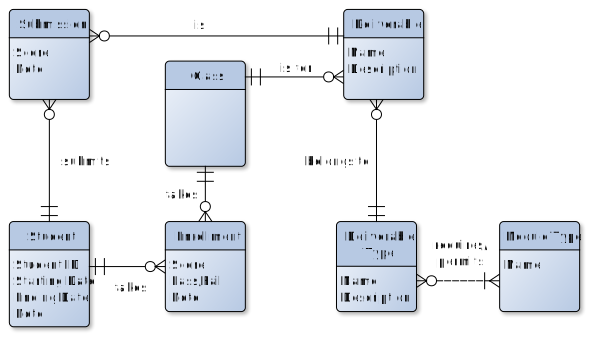
\includegraphics[scale=0.6]{\currentDir/erdDeliverables1}%
\caption{The handling of deliverables in our teaching management platform.}%
\label{fig:erdDeliverables1}%
\end{figure}%
%
Another part for our platform will focus on deliverables in \cref{fig:erdDeliverables1}.
There are different types of deliverables, e.g., written exams, oral exams, midterm exams, homework, internship reports, or theses.
Each module type may require any number of deliverables of different types.
Each module type may also permit any number of deliverables.
(We modeled these two relationships as one to save space.)
We already have established that classes belong to modules belong to module types.
So from the relationship between module types and deliverable types, we can infer what deliverable types are permitted and/or required for every class.
For a Master's Project, a Master's Thesis may be a required deliverable.
For a course \inQuotes{Databases}, a written final exam may be required and a mid-term exam as well as homeworks may be permitted.
The teacher then will create a (weak) \emph{Deliverable} entity, which has a Name and a Description.
Each students will make corresponding submission for the deliverable.
These submissions will not go to our platform.
Instead they are sent to the teacher.
The teacher evaluates them and creates the corresponding (weak) \emph{Submission} entities -- one per student -- in the system.
This weak entity holds the result of the student and maybe a comment by the teacher.
This way, the teacher can upload exam results, mid-term exam results, and so on.
The students then can view them in the online system.
Notice that we here just wrote \emph{Score} as attribute, but we may as well imagine that other attributes like pass/fail would make sense here.

\begin{figure}%
\centering%
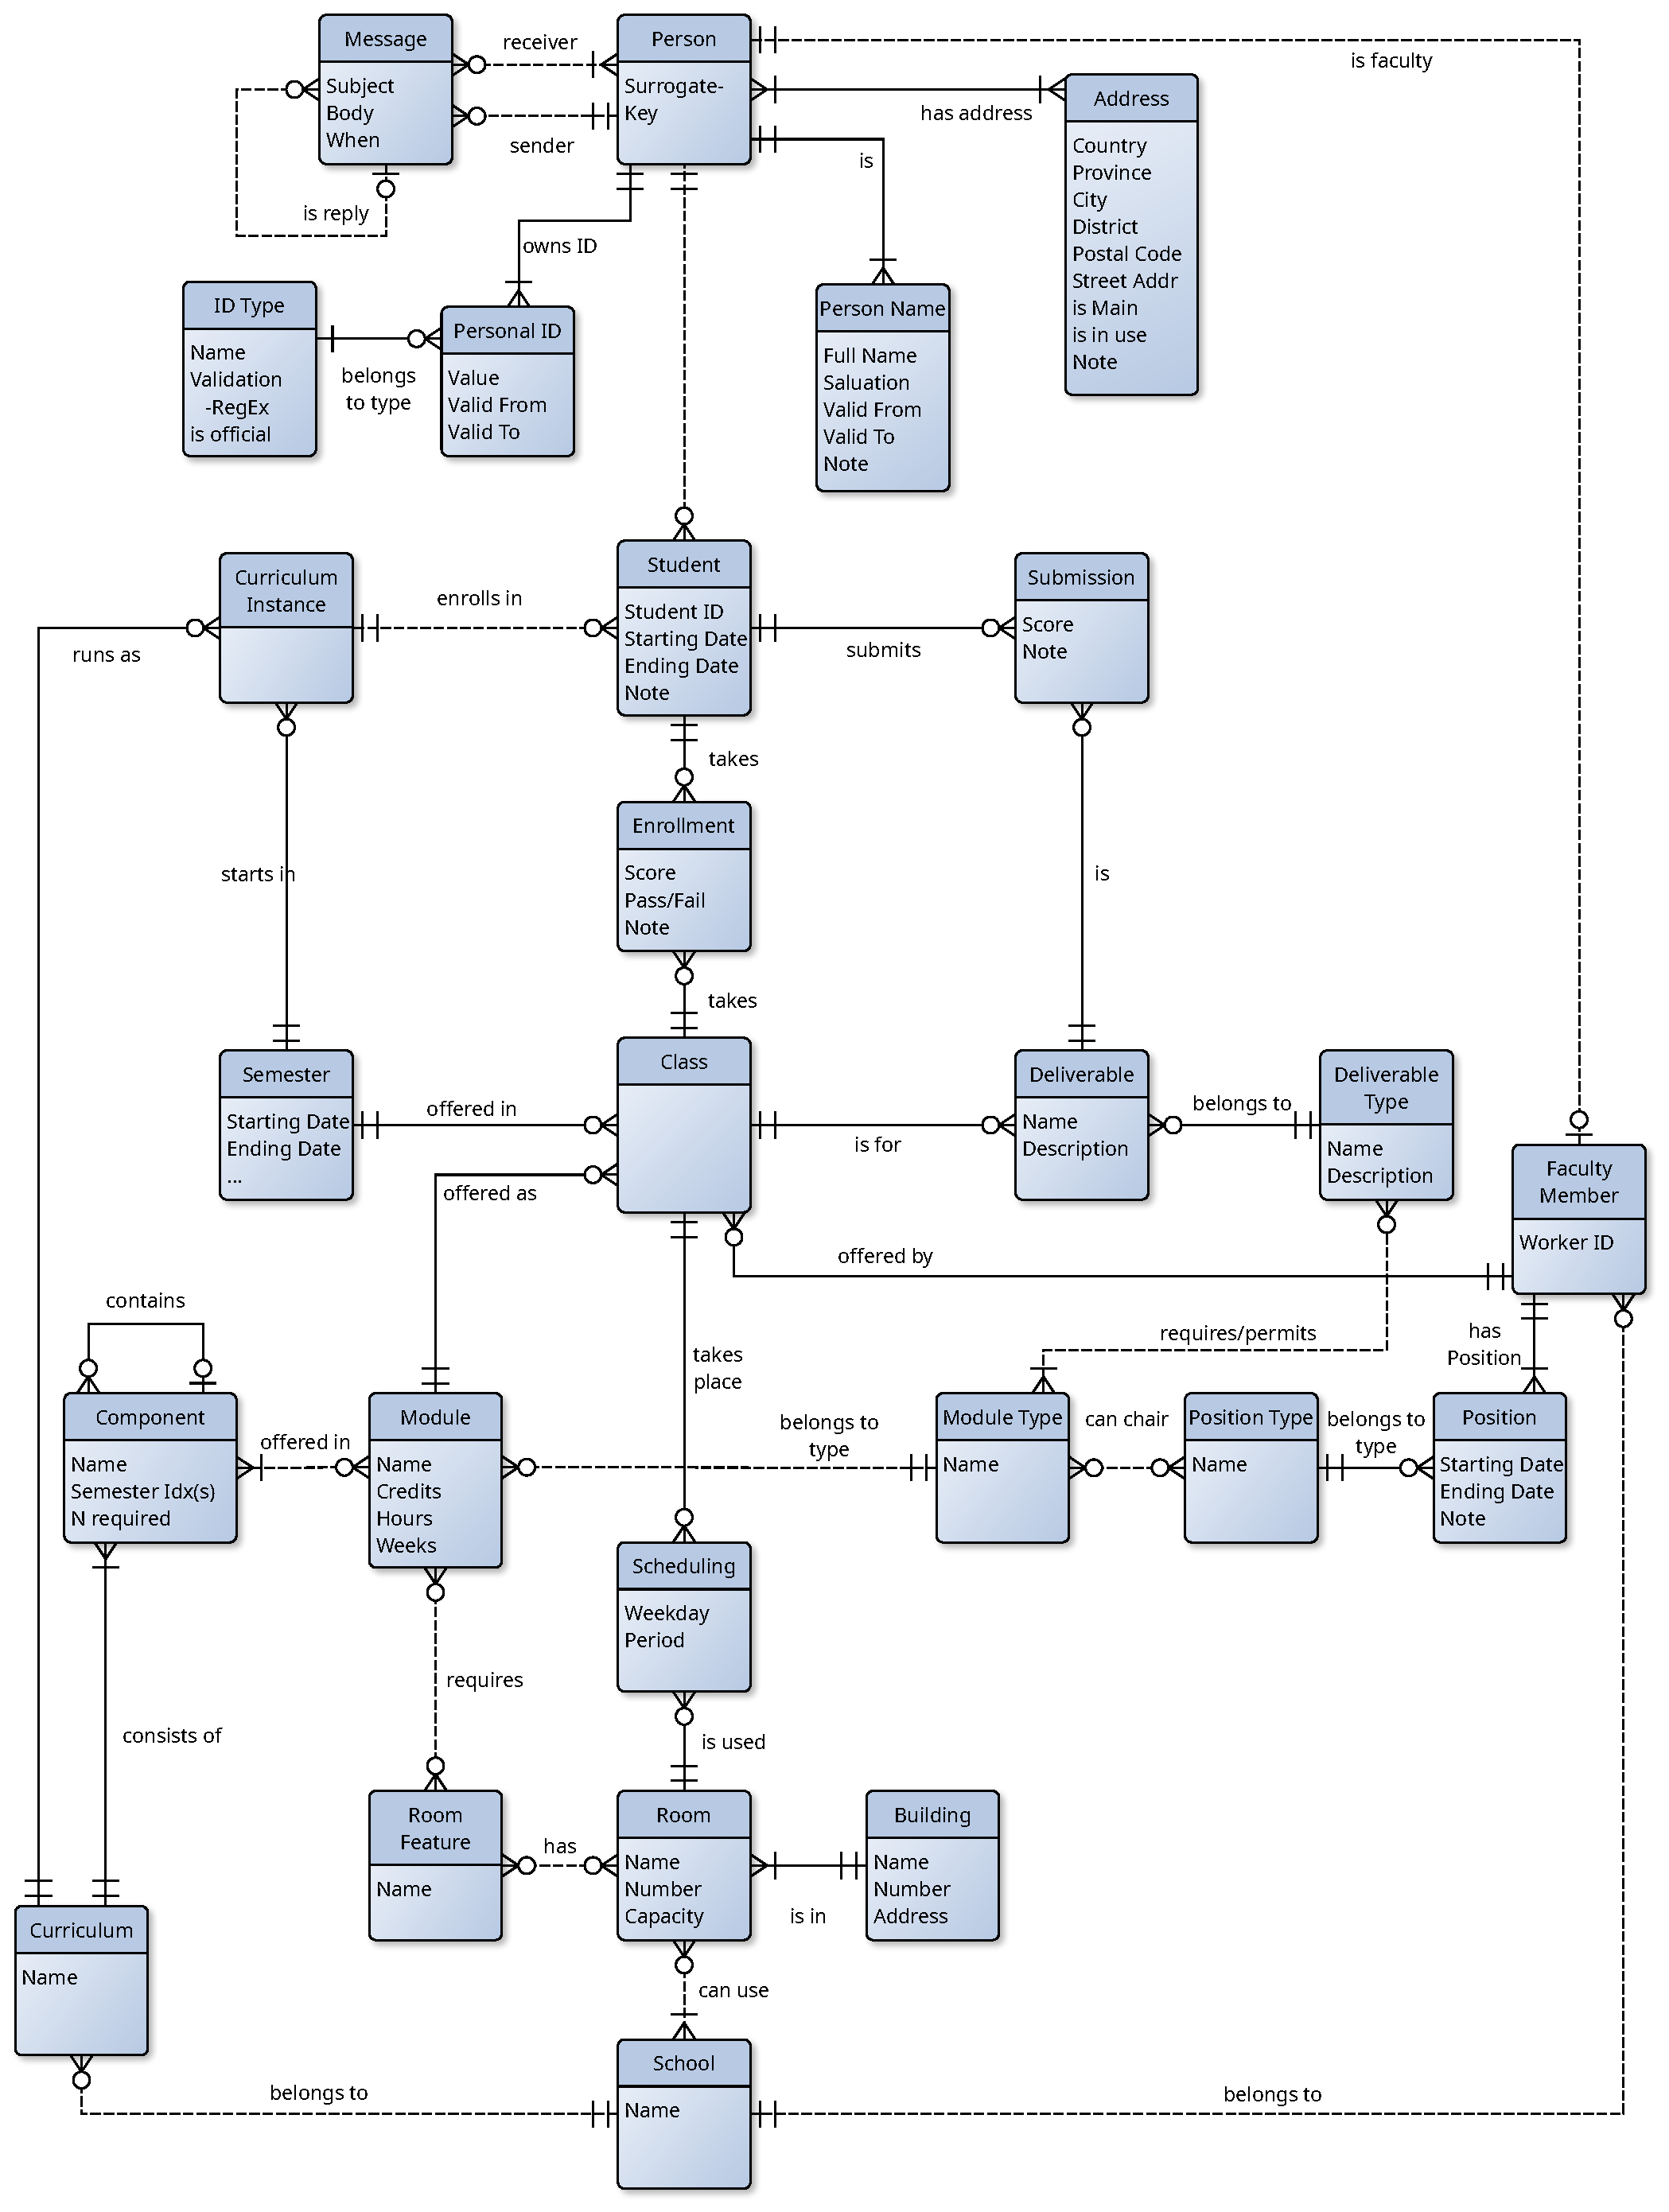
\includegraphics[width=0.99\linewidth,height=0.8\textheight,keepaspectratio]{\currentDir/erdPlatform1}%
\caption{A complete overview of the conceptual model of our teaching management platform.}%
\label{fig:erdPlatform1}%
\end{figure}%
%
All of the elements of this conceptual draft of our teaching management \db\ are included in \cref{fig:erdPlatform1}.
This model is still not very advanced.
But it has already several good features.
We can imagine that it will be at least somewhat usable.

We did not explicitly state this before, our model for the teaching platform partially follows the principle of an \emph{Insert-Only Database}~\cite{P2014ACIIMDMTIMOIMD:IO}:%
%
\bestPractice{immutableData}{%
In many application scenarios where historical information needs to be preserved, data in a \db\ should never be changed or deleted. %
Changes in the real world should instead be reflected by adding data to the \db.}%
%
In other words, viewing this from the \sql\ perspective, \sqlil{UPDATE} and \sqlil{DELETE} operations should not be used if we need to remember the past state of data.
Instead, only new records should be added via \sqlil{INSERT INTO}.
And in our situation, we do want to preserve the history of the data.

For example, a curriculum consists of modules.
Now we could have modeled that each module is assigned to a teacher.
Once the teacher changes their workstation and another teacher takes over, we could just change the assignment.
This would be much simpler than our current conceptual model.
It would have a big drawback, though:
It would be impossible to tell which teacher taught a module in the past.

Therefore, we chose a different path:
Each instantiation of a module is a class and each class is assigned to a teacher.
This assignment never changes.
Each semester, new class records are added.
We always know who taught which course in which semester.
Our \db\ will grow incrementally an changes are reflected by new records and not the modification of existing records.
If a module is taken over by another professor, then this will yield a new class instance.
We can see who taught which class (module) in which semester.

For this reason, we also added the \emph{Valid From} and \emph{Valid To} attributes to the \emph{Address} entity type.
If the address of a student or faculty member changes, we create a new address record and mark it as valid starting today, while leaving the \emph{Valid To} attribute at \sqlil{NULL}.
We then enter yesterday as \emph{Valid To} value of the old address as no longer in use.
The same also holds for our \emph{Personal ID} and \emph{Person Name} entity types.
The administrators can therefore immediately see which address, ID, or name a person had in use when some action was taken in the past.

Our system also has some shortcomings.
For example, there may be some more levels of structural indirection in a university.
A school may be subdivided into different departments.

Furthermore, we should be able to add timestamps and notes to most of the data items, which we did not really model here.
Also, we did not model rights management.
We would probably need a table assigning which person is permitted to enroll students into a class or curriculum, which person in a school can create new modules, classes, curricula, and so on.
Or we could also handle this via the position submodule that we already designed.
This would probably a good idea.

Additionally, we may want to create a table creating an audit trail~\cite{K2010ATTDCID}.
Such a table would store which user added/changed which record in which table at which point in time.

Finally, in our \emph{Address} entity, countries and provinces are simple attributes.
We could probably have another entity type to represent countries and country subdivisions (such as provinces) based on the ISO~3166 standard~\cite{ISO3166}, maybe with additional information such as the phone number prefix.
Each address could be linked to at least one such entity via a relationship.

For now, we omit all of this.
Such features could probably be added later.
The system looks more or less reasonable, so our goal is to move on to create a logical model and then a prototype.%
%
\FloatBarrier%
\endhsection%
%
